\documentclass[12pt]{article}
\usepackage[english]{babel}
\usepackage{natbib}
\usepackage{url}
\usepackage[utf8x]{inputenc}
\usepackage{amsmath}
\usepackage{graphicx}
\graphicspath{{images/}}
\usepackage{parskip}
\usepackage{fancyhdr}
\usepackage{vmargin}
\usepackage{xcolor}
\usepackage{siunitx}
\usepackage{physics}
\setmarginsrb{3 cm}{2 cm}{3 cm}{2 cm}{1 cm}{1.5 cm}{1 cm}{1.5 cm}

\title{Lab 03}													% Title
\author{G 03}														% Author
\date{2 Apr 2019}														% Date

\makeatletter
\let\thetitle\@title
\let\theauthor\@author
\let\thedate\@date
\makeatother

\pagestyle{fancy}
\fancyhf{}
\rhead{\theauthor}
\lhead{\thetitle}
\cfoot{\thepage}
\newcommand{\mis}[3]{(#1 \pm #2) \ #3}
\newcommand{\misp}[3]{(#1 \#3 \pm #2}
\begin{document}

%%%%%%%%%%%%%%%%%%%%%%%%%%%%%%%%%%%%%%%%%%%%%%%%%%%%%%%%%%%%%%%%%%%%%%%%%%%%%%%%%%%%%%%%%

\begin{titlepage}
	\centering
    \vspace*{0.5 cm}
    
\includegraphics[scale = 0.75]{polito.jpg}\\[1.0 cm]				% University Logo
    \textsc{\LARGE Politecnico di Torino}\\[2.0 cm]						% University Name
	\textsc{\Large Digital systems electronics\\ A.A. 2018/2019}\\[0.5 cm]		% Course Code
	\textsc{\Large Prof. G. Masera}\\[0.5 cm]		% Nome del Professore
	\rule{\linewidth}{0.2 mm} \\[0.4 cm]
	{ \huge \bfseries \thetitle \\ \small \thedate}\\
	\rule{\linewidth}{0.2 mm} \\[1.5 cm]
	
	\begin{minipage}{0.4\textwidth}
		\begin{flushleft} \large
			Berchialla Luca\\												%Cognomi e nomi
			Laurasi Gjergji
			\\
			
			Mattei Andrea\\
            Lombardo Domenico Maria\\
            
			\end{flushleft}
			\end{minipage}~
			\begin{minipage}{0.4\textwidth}
            
			\begin{flushright} \large
			236032\\													%Matricole
			238259\\
            233755\\
            233959\\
            
		\end{flushright}
        
	\end{minipage}\\[2 cm]
	
\end{titlepage}

%%%%%%%%%%%%%%%%%%%%%%%%%%%%%%%%%%%%%%%%%%%%%%%%%%%%%%%%%%%%%%%%%%%%%%%%%%%%%%%%%%%%%%%%%

\section{4-bit Sequential RCA}

\begin{figure}[h]
	\centering
	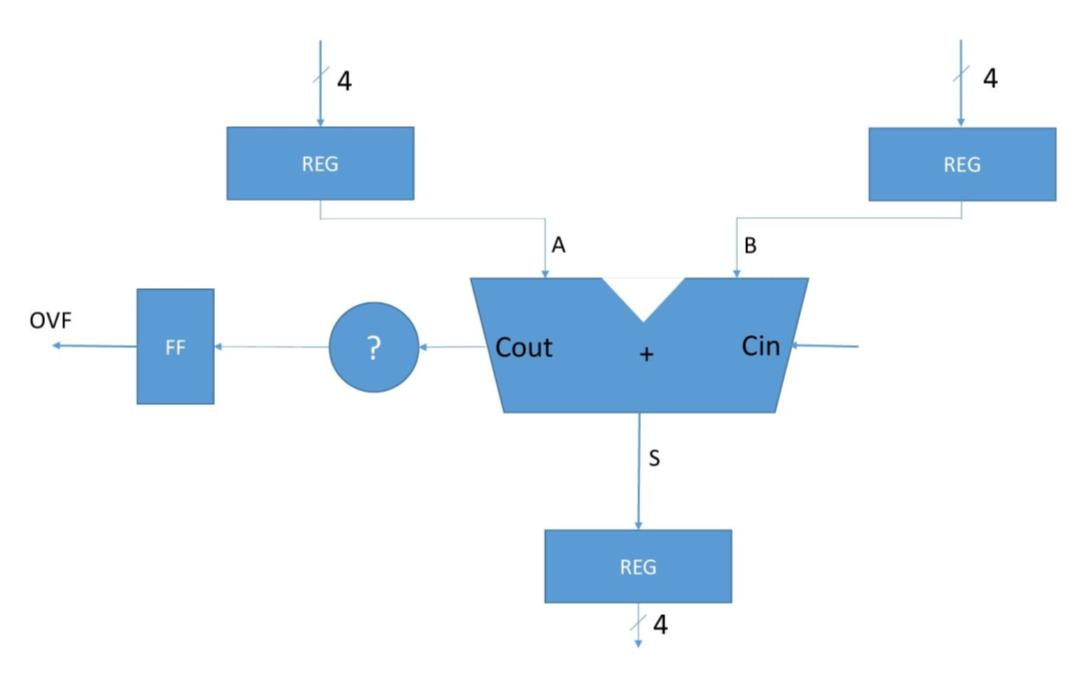
\includegraphics[scale = 0.8]{immagini/B1.jpg}
	\caption{Top level entity}
\end{figure}


Here we had to implement a 4-bit Sequential Ripple Carry Adder. To build the circuit requested in $figure 1$ several sub-circuits have been implemented.\\
As first point a Full Adder was implemented as shown in $figure$ $2a$. The 4-bit adder was built using four full adders in a ripple carry architecture. Its overflow signal is generated by a $xor$ gate whose inputs are the $carry_{out}$ signals of the last two full adders.\\

\begin{figure}[h]
	\centering
	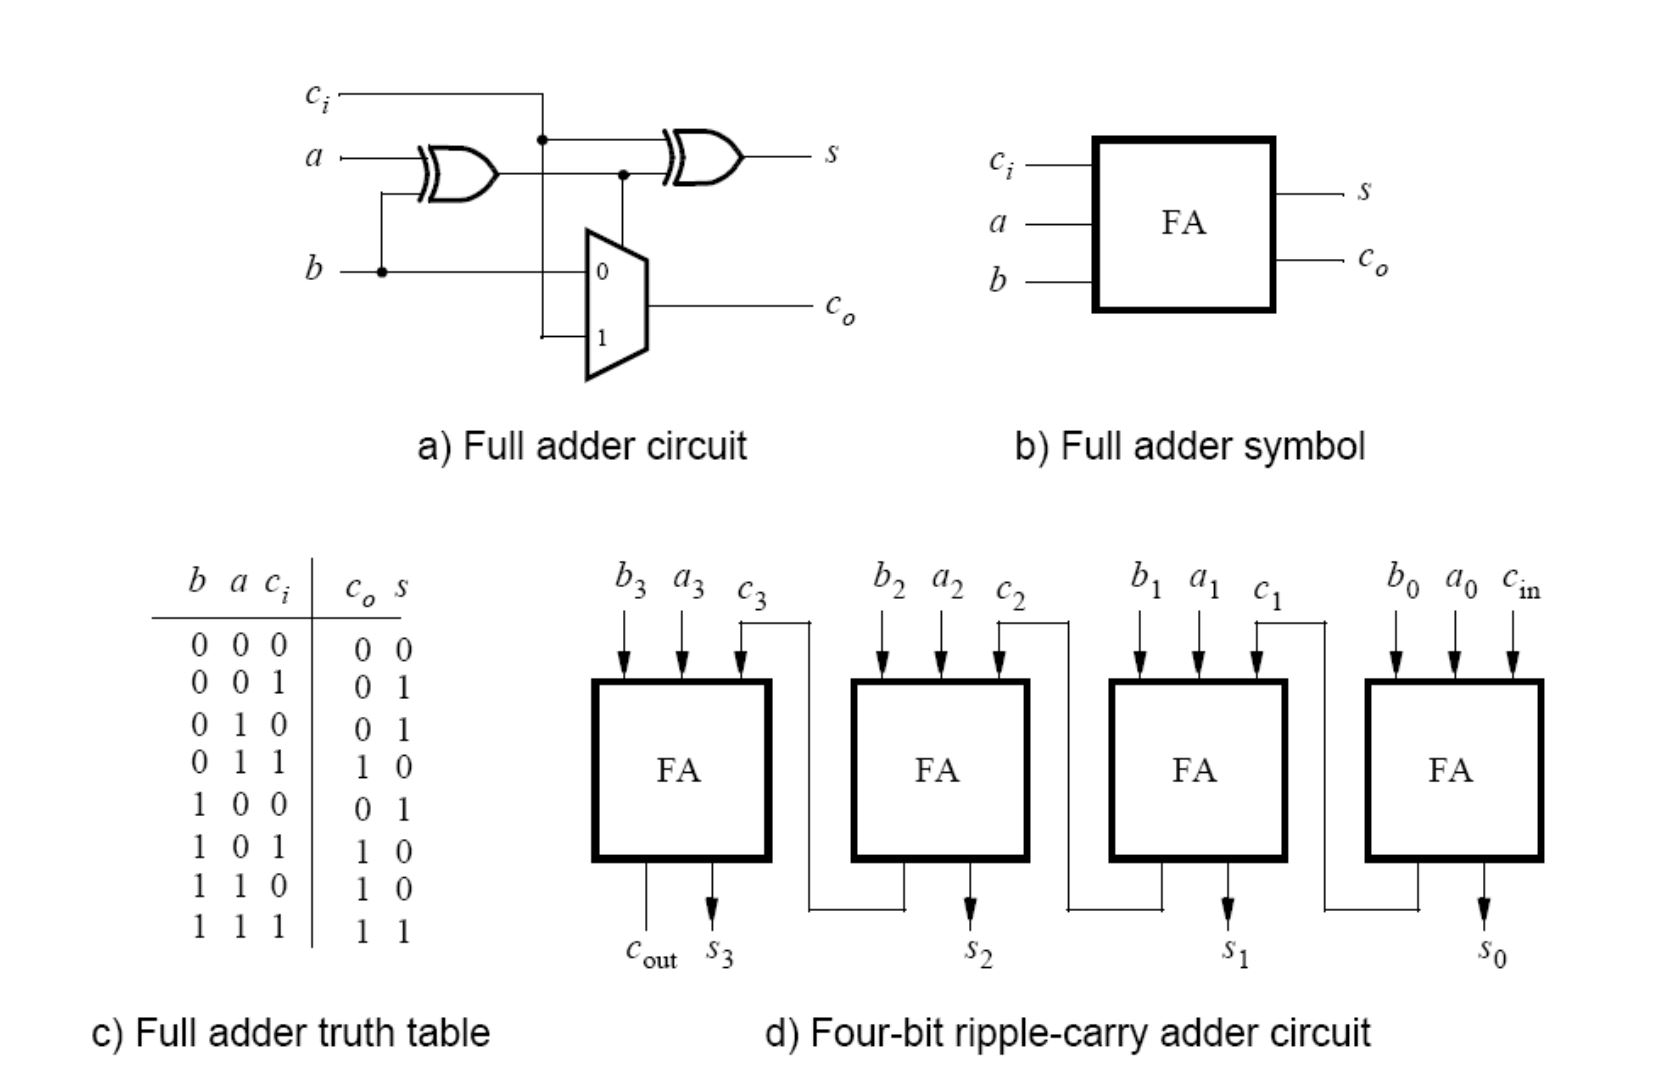
\includegraphics[scale = 0.4]{immagini/B2.jpg}
	\caption{Full Adder}
\end{figure}

The Register and the Flip-Flop were implemented using the code provided in the instructions.\\
A new 7-segments display decoder was needed in order to display properly 2's complement numbers. It uses two 7-segments displays to show respectively the sign and the magnitude of the number. The implementation was done by means of the $when-else$ statement following the truth table in $figure$ $3$.
\begin{figure}[h]
	\centering
	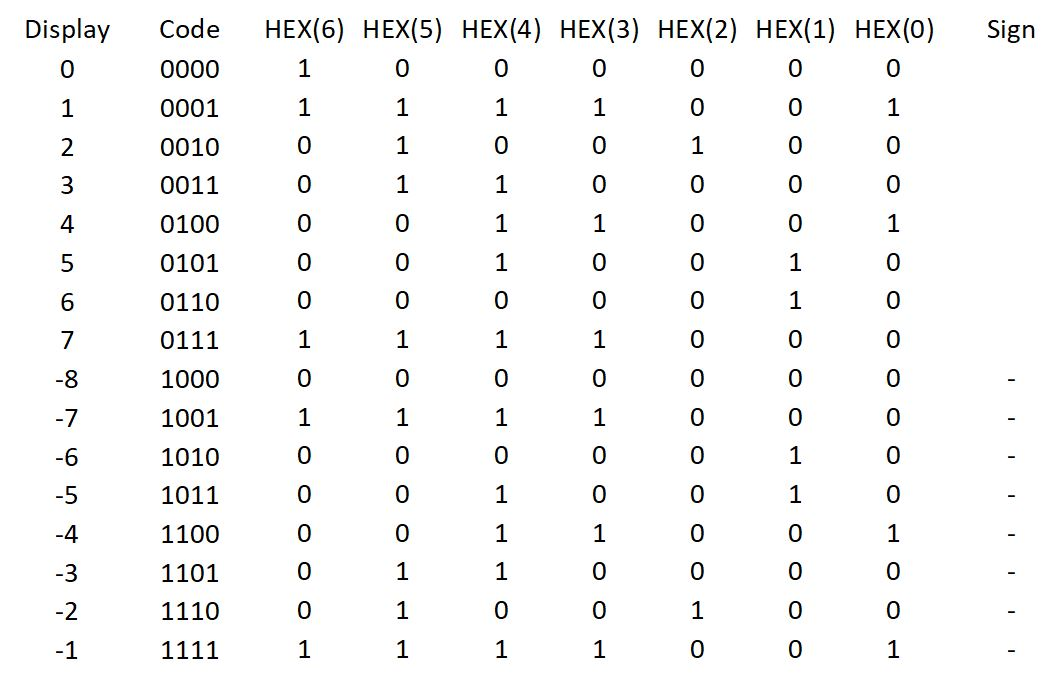
\includegraphics[scale = 0.7]{immagini/B3.jpg}
	\caption{2's complement 7-segments decoder}
\end{figure}\\
The top level entity that implements the circuit is in the file $lab3\_es1.vhd$ where all the components needed........





\section{4-bit Sequential Adder/Subtractor}

	


\section{3}
punto 3


\section{4}
punto 4

\end{document}
